% !TEX encoding = IsoLatin
\documentclass[11pt]{report}
\usepackage{graphicx}
\usepackage[latin1]{inputenc}
\usepackage[T1]{fontenc}
\usepackage[french]{babel} 
\usepackage{setspace}
\usepackage{cite}
\usepackage{lscape}
\usepackage{fancyhdr}
\usepackage{xcolor}
\usepackage[acronym, toc]{glossaries}
\usepackage[export]{adjustbox}
\usepackage[a4paper, left=2cm,right=2cm,top=2cm,footskip=1cm,bottom=2cm]{geometry}
\usepackage{hyperref}

\geometry{% margin settings
    paper=a4paper, 
    inner=2.0cm, % Inner margin
    outer=2.0cm, % Outer margin
    bindingoffset=0.0cm, % Binding offset
    top=2.0cm, % Top margin
    bottom=2.0cm, % Bottom margin
    includeheadfoot,
    headsep=5mm,
    footskip=1.8cm
}

\setlength{\headheight}{14pt}
\fancypagestyle{plain}{
\fancyhead[L]{Dossier entreprise}
\fancyhead[R]{Matthieu Balondrade - MSI 2019}
\fancyfoot[L]{
\includegraphics[width=3cm]{cesi.png}}
\fancyfoot[R]{
\includegraphics[width=3cm]{docdoku.png}}}
\definecolor{burntorange}{RGB}{211, 84, 0}


\pagestyle{plain}

\title{\Huge \color{burntorange}{Dossier entreprise Docdoku}}
\author{\Large Matthieu \bsc{Balondrade} \\ MSI 2019 }
\date{\Large 5 Février 2020}

\begin{document}
\begin{titlepage}
	\centering
	
\includegraphics[width=0.3\textwidth]{cesi.png}\par\vspace{1cm}
	{\scshape\Large MSI 2019\par}
	\vspace{3cm}
	{\huge\bfseries \color{burntorange}{Dossier entreprise}\par}
	\vspace{2cm}
	{\Large\itshape Matthieu Balondrade\par}\vspace{2cm}
	\vfill

% Bottom of the page
	
\includegraphics[width=0.3\textwidth]{docdoku.png}\par\vspace{2cm}\par
	{\large 5 Février 2020\par}


\end{titlepage}
\tableofcontents

\part{L'entreprise}

	\chapter{Organisation}

		\section{Les services}

			L'entreprise est organisée autour de 5 services:\\

			\begin{description}
				\item[Administratif: ]Le service administratif interne permet de gérer la relation entre l'entreprise et le personnel de celle-ci. 
			Laurie \bsc{Pujos}, la responsable du service, est présente pour apporter toutes les ressources nécessaires
			au bon fonctionnement du service.
			Ce service apporte le domaine comptable, la gestion juridique, et l'approvisionnement. 
				\item[Gestion de projet: ] Les différents membres de la gestion projet sont chargés de veiller au bon fonctionnement des projets sous leurs responsabilité.
				\item[Management: ] Eric \bsc{Descargue}, responsable du service Management et fondateur de la société maintient l'organisation et la distribution des ressources humaine. Ce service est fondateur des relation inter-personnelles
			professionnelle dans l'entreprise. 
				\item[Relation client: ] Les clients de Docdoku passent par se service pour consulter et accéder aux différents produits. Formations, prestation informatique, suivi de projet. Les différents membres de ce service sont à l'écoute
			de parties prenantes externes actuelles et futures.
				\item[Technologies: ] Chez Docdoku, l'effectif est concentré dans le service technologique. Du fait des missions, des prestations de formations et de l'outil open source qu'elle propose, elle dispose de membres polyvalent 
			se pretant aux différents besoin en matière de développement logiciel. Ce service est géré par Florent \bsc{Garin}, fondateur de Docdoku.
			\end{description}

		\newpage

		\section{Localisation}

			Les locaux de docdoku sont situé en plein centre de toulouse dans l'avenue jean jaurès

				\begin{figure}[!htb]
					\center
					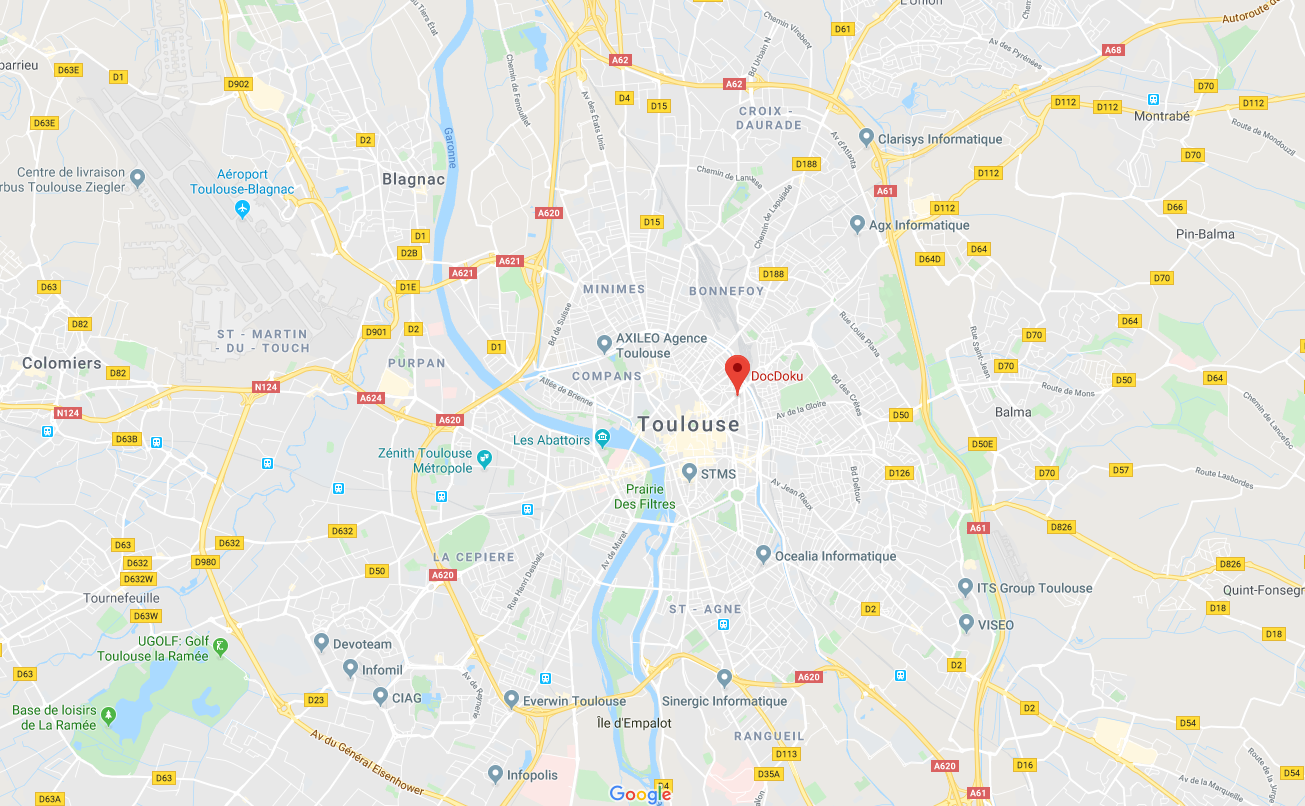
\includegraphics[scale=0.3]{local.png}
					\caption{Docdoku, 76 Allée Jean Jaures, 31000 Toulouse}
				\end{figure}

		\section{Organigramme}

			\begin{landscape}
				\begin{figure}[!htb]
				\center
				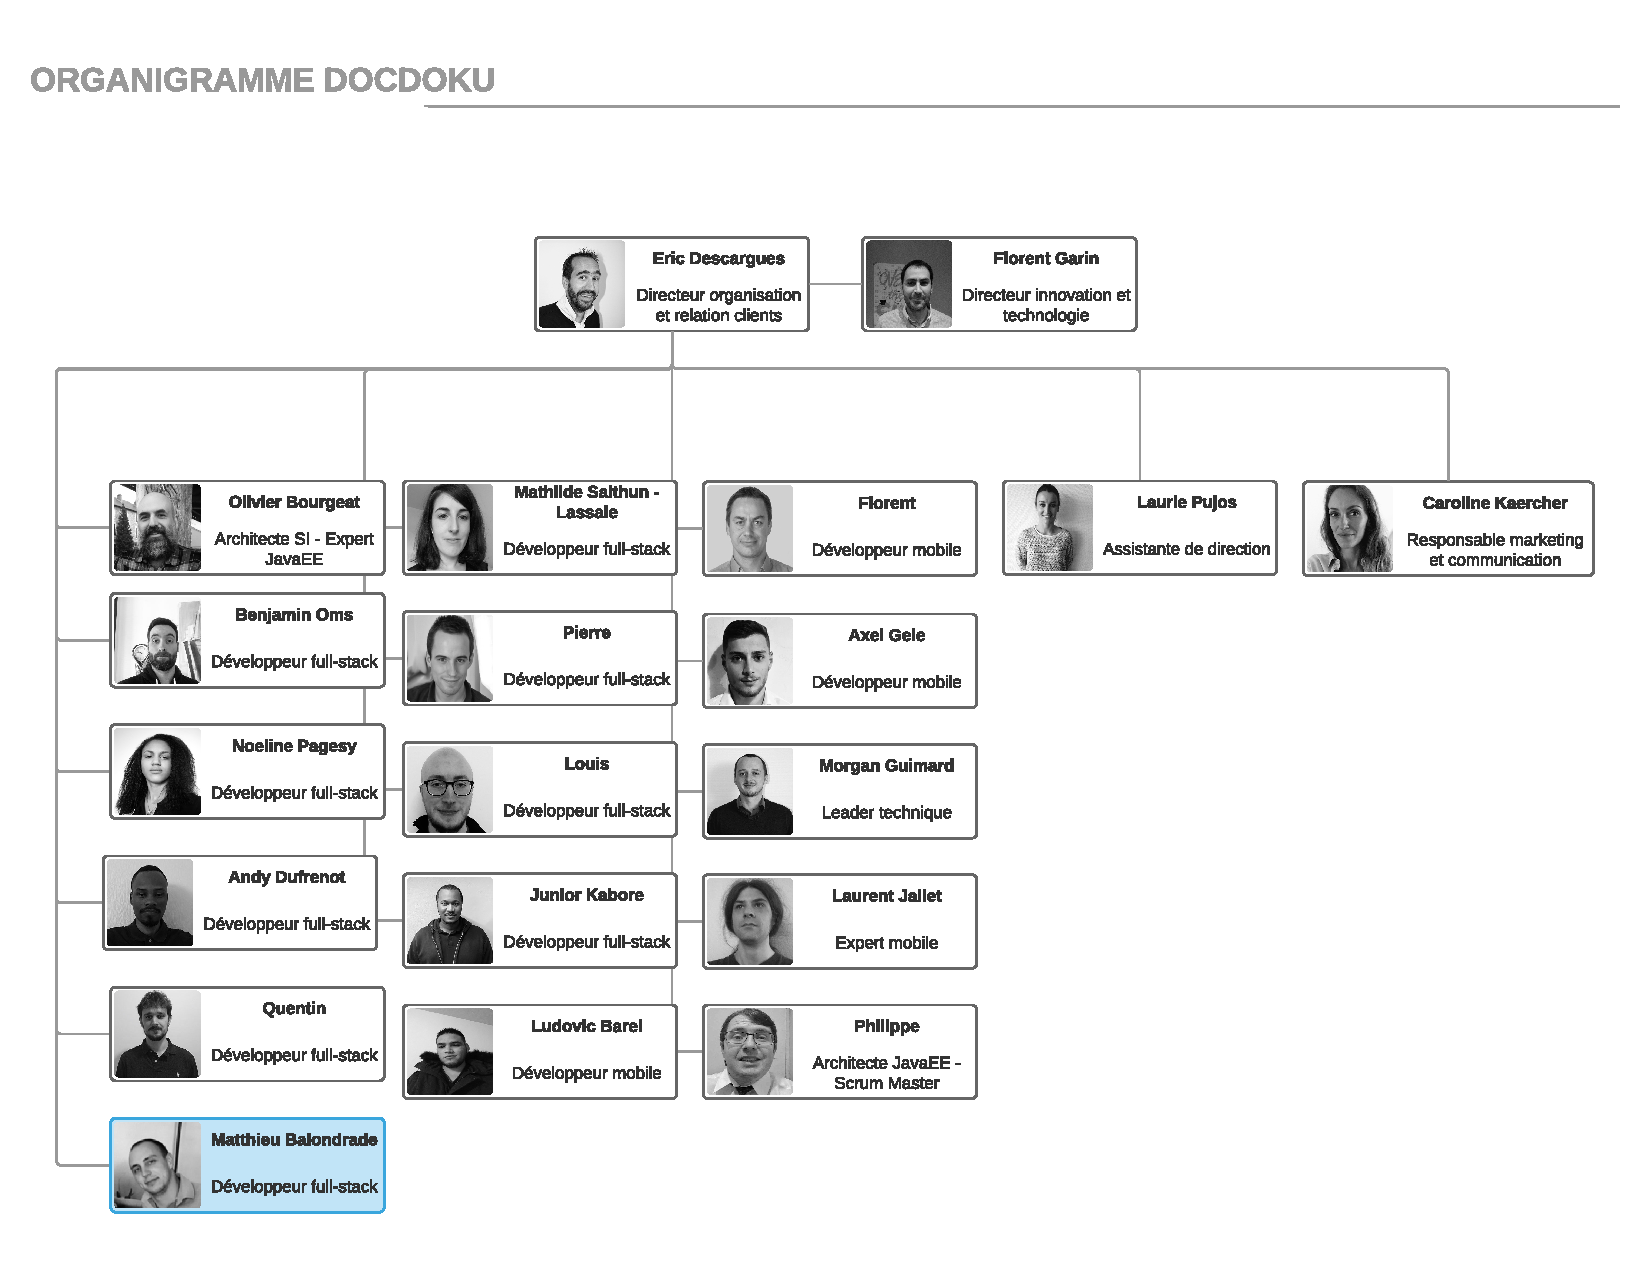
\includegraphics[scale=0.75]{Organigramme.pdf}
				\caption{Organigramme de Docdoku}
				\end{figure}
			\end{landscape}

	\chapter{Missions}

		Docdoku est une entreprise créatrice de solution digitales métier. Impliquée dans l'Open Innovation, elle développe DocDokuPLM , une plateforme Open Source de Business Data Management qui facilite la gestion des données des entreprises.\\
		Son secteur est celui des Technologies de l'Information et de la Communication (TIC ou ICT).\\
		Elle dispose d'une expertise technique dans les domaines du Web, Mobile/Tactile, du Système d'Information et en propose des formations. 
		Sa mission est d'aider les organisations à digitaliser leur métier.\\
		Elle reçoit des demandes d'applications digitales métier, supportant ses composants Open Source et réalise des formations à ces technologies.
		Partenaire avec de nombreuses grandes entreprises et groupes comme :

		\begin{description}
			\item[Airbus : ] Dans la formation aux langages frontend et sur l'architecture logicielle web. Egalement Docdoku a réalisé une mission de développement logiciel utilisant sa plateforme DocdokuPLM
			\item [Air France : ] Afin de répondre à un projet client, Air France a consulté Docdoku pour la montée en compétences de ses collaborateurs dans les domaines du développement Android. Elle a également réalisé un projet mobile chez Docdoku
			\item [Continental :] Réalisation d'une application mobile multiplateformes embarquée permettant une aide à la conduite.
			\item [SNCF :] Réaliser l'audit de l'application TER mobile et recommander les actions qui en incombent, mener l'étude technique préalable et chiffrer le projet d'application tactile pour agents d'escales
		\end{description}

		\singlespacing
		\noindent
		Elle est également présente pour l'étranger auprès de gros groupes: 

		\begin{description}
			\item [Honeywell: ] Pilotant les capteurs photos, l'API Camera d'Android a évolué et présente une nouvelle génération : Camera2. DocDoku a effectué la mise à jour iso-fonctionnelle sur la derniere version du SDK (Software development Kit) permettant à ses clients de se connecter à ses systèmes.
		\end{description}

		\section{Quelques missions importantes confiés à Docdoku}

			\subsection{Amazon}
				Amazon était à la recherche d'une solution de Product Lifecycle Management (PLM) et avait entrepris de consulter les principales plateformes open source disponibles sur le marché.
				\singlespacing
				Le fait que l'architecture de DocDokuPLM soit autoscalable et s'adapte aux montées en charge de centaines de milliers d'utilisateurs a été différenciant.
				La plateforme a également réussi son examen de passage quant aux aspects sécurité, Amazon ayant réalisé un audit complet du code avant sa prise de décision finale. Enfin, l'approche « Sandbox » proposée par DocDoku, permettant une mise en production rapide en mode Agile, a fini de retenir l'attention du géant du web.
				La Team DocDoku a donc déployé DocDokuPLM sur une infrastructure cloud AWS (sans surprise;), accompagnée de développements complémentaires pour répondre à ses spécificités métier.
				Amazon a en outre souhaité que ces développements restent dans le domaine open source pour bénéficier des éventuelles évolutions apportées par la communauté.

			\singlespacing

				Nous avons travaillé en étroite collaboration avec Airbus, en nous appuyant sur notre plate-forme DocDokuPLM. Nous avons ainsi construit une solution sur mesure intégrée à l'environnement de l'industriel qui est composé de différents systèmes PLM et qui repose en ce qui concerne l'aspect CAO sur Catia de Dassault Systèmes.

			\subsection{Airbus}
				L'applicatif déployé se base uniquement sur les technologies standard du Web grâce auxquelles le service est disponible depuis n'importe quel OS bureautique (Windows, Mac et Linux), ainsi que depuis les systèmes mobiles. \\
				Une chaîne sophistiquée de traitements, déployée sur une grille de calcul, importe les modèles 3D Catia et les métadonnées associées pour pouvoir être ensuite affichés sur un simple navigateur web sans plugin.\\
				A l'aide des Web Services et API JavaScript, nous avons créé des applications mashup qui mixent données PLM, modèles 3D et du contenu provenant de logiciels hétérogènes.

			\singlespacing

				\begin{figure}[!htb]
					\center
					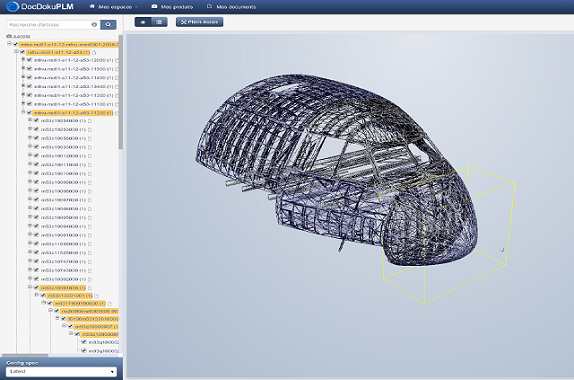
\includegraphics{a1.png}
					\caption{Product Structure Avion}
				\end{figure}

			\subsection{Air France}

				\paragraph{Besoin\\}
				Air France a réalisé en 2013 l'application mobile AF Press permettant à ses passagers de télécharger et de lire des journaux et magazines au format pdf sur leurs propres tablettes. Il s'agissait pour 2015 de lancer la version 2.0 de cette application avec une interface revisitée, une compatibilité élargie aux smartphones, l'optimisation de l'utilisation de la mémoire vive, et supportant le plus large éventail d'appareils Android possible.

				\paragraph{Solution\\}
				Une toute nouvelle application native a été créée et sera disponible sur le Play Store rapidement. Toutes les tailles d'écran et toutes les densités sont supportées. L'application est disponible à partir d?Android 4.0 (Ice Cream Sandwich) ce qui couvre plus de 90\% des appareils.

				\begin{figure}[!htb]
					\center
					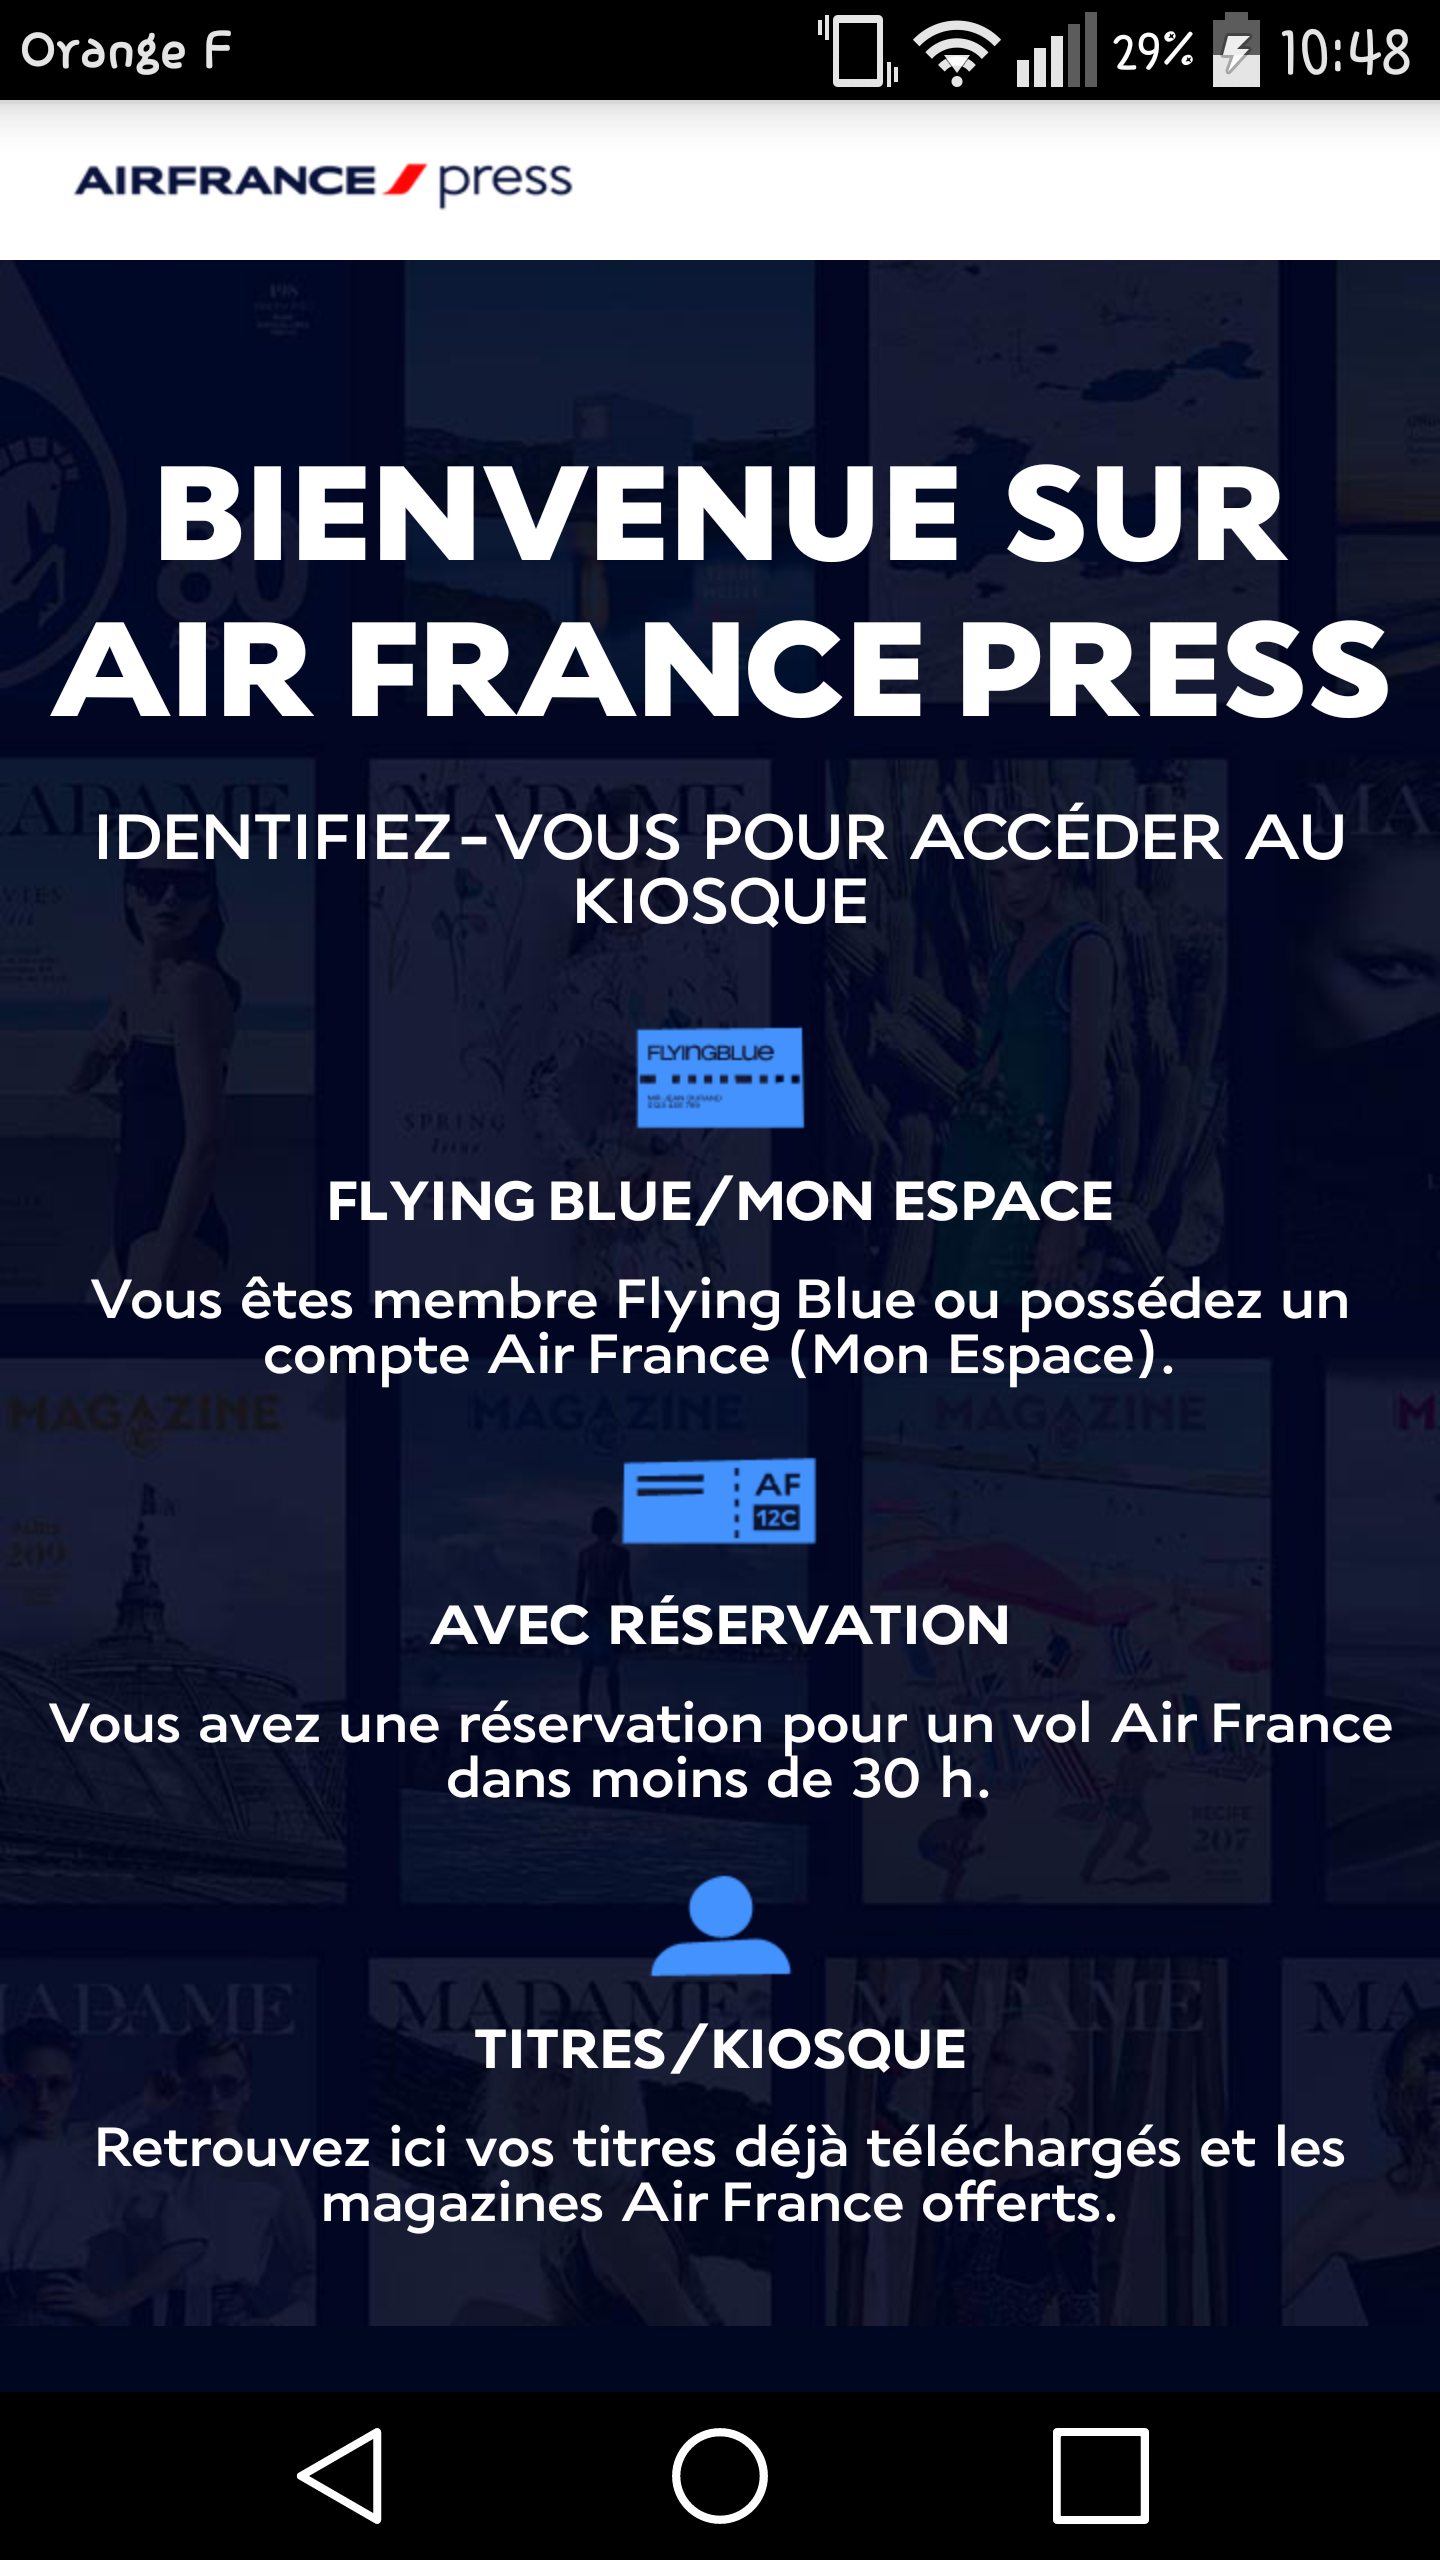
\includegraphics[scale = 0.15]{mb1.png}
					\caption{Home page de l'application presse Air France}
				\end{figure}

	\chapter{Communication}

		\paragraph{Communication externe\\}
			Convaincus que pour inventer il faut s'ouvrir au monde extérieur, Docdoku partage quotidiennement ses expériences et compétences au travers d'ouvrages, de contributions Open Source, de son blog ou de nombreux événements et séminaires auxquels elle participe.\\
			C'est évidemment pour obtenir et garder la confiance de ses client qu'elle met tout ceci en oeuvre.

		\begin{figure}[!htb]
			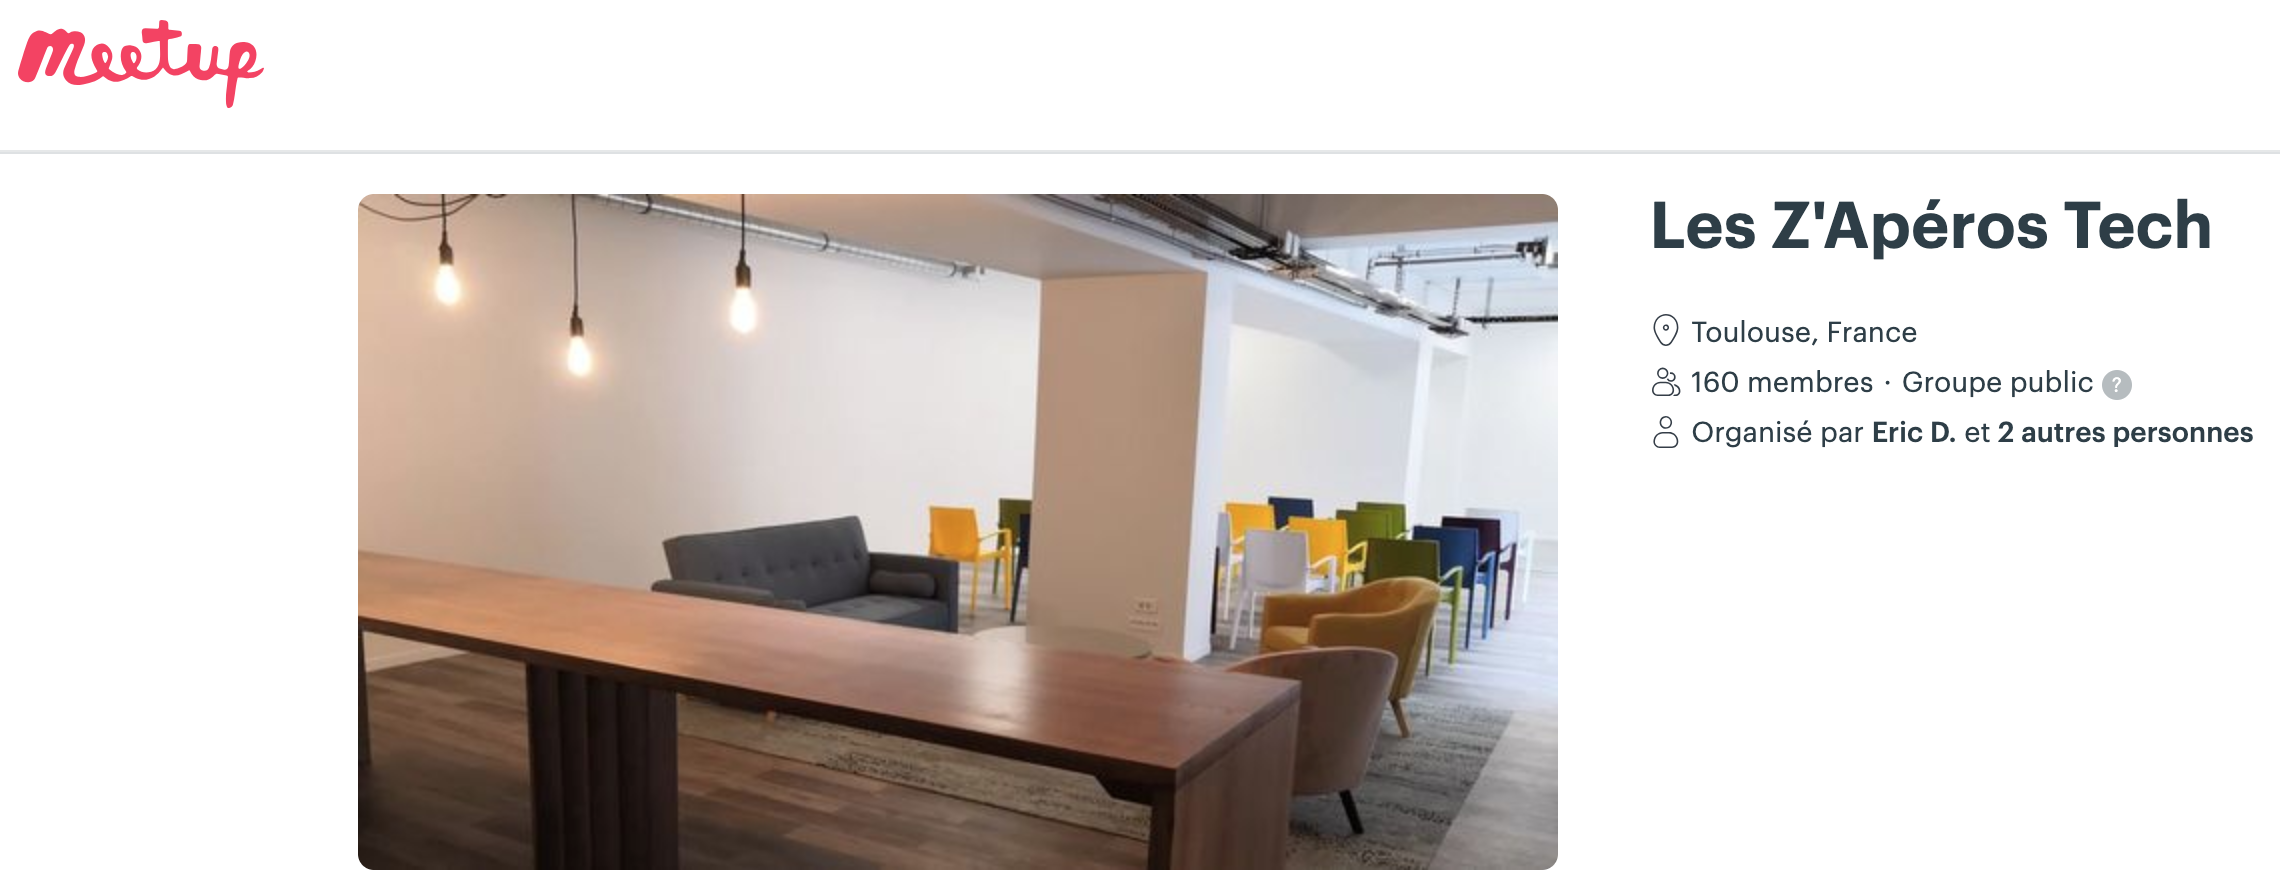
\includegraphics[scale = 0.4,left]{meetup.png}
			\caption{Évènement Meetup à Docdoku}
		\end{figure}

		\paragraph{Communication interne\\}
			Afin de collaborer au sein de l'entreprise, Docdoku à mis en place divers outils et techniques de communication.

		\section{Le management agile}
			Certaines méthodes dans le management de projet Agiles permettent une meilleure communication au sein de l'équipe. \\
			Les Sprints planning pour organiser les tâches des prochains jours.\\
			Le plannings pokers permettant de communiquer sur l'ordre et la difficulté de réalisation des tâches, sprint review.

		\newpage
		\section{Les outils}
			Docdoku met à dispositions divers outils pour communiquer au sein de l'entreprise.

			\begin{description}
				\item[Google suite :] L'entreprise Docdoku fait bénéficier à tout ses employés un compte google + permettant de communiquer par le biais de mail, partage de document, et communauté interne.
				\item[Slack :] A travers cet outils, plusieurs communication au sein des différents projets et activités de l'entreprise ont lieux. Nous avons également les notifications d'autres outils tel que l'intégration continue avec Jenkins® et Gitlab® .
				\item[Hangout :] C'est l'outils de communication, individuelle principalement, par excellence. Les membres peuvent interagir par le biais de messages écris et appels Visio.
				\item[OpenSpace :] La disposition de l'entreprise met en avant la communication par l'open space. Bien qu'il présente le risque d'une communication bruyante, les employés peuvent interagir rapidement entre eux.
			\end{description}

\part{Ma place au sein de la DSI}

	\chapter{Mon positionnement}

		Je suis employé chez Docdoku en tant que Développeur logiciel Full-Stack. Bien que j'appartienne au service technologique, il n'y a pas de hiérarchie précise au sein de l'entreprise.\\

		Je suis rattaché à mon tuteur Florent \bsc{Garin} qui peux m'apporter de l'aide dans le domaine de connaissance Technique et Management ainsi qu'au Lead-Developpeur Morgan \bsc{Guimard}, plus spécialisé en développement logiciel.\\

		Actuellement au sein d'une équipe de 5 personnes pour le projet qui m'a été confié les membres de l'équipe sont définis comme suit:\\
		\begin{description}
			\item[Noëline \bsc{Pagesy} \& Guangjie \bsc{Zhang} \& Rémi Buhler :] Développeur(se) IOS 
			\item[Andy \bsc{Dufrenot}:] Développeur Android \& Frontend
			\item[Matthieu \bsc{Balondrade}:] Développeur Backend \& Scrum Master
		\end{description}

	\chapter{Mes missions en entreprise}

		\section{Projet Honeywell}

			Je suis chargé de la réalisation de différents projets confié à l'entreprise Docdoku.\\

			Actuellement il m'a été confié la réalisation d'un projet nommé SwiftDecoder Wedge auprès de notre client Honeywell.\\

			Ma mission consiste à la réalisation d'une application de scan de code d'identification comportant différents mode, scan multiple, choix de la source, scan selon des critères spécifiques.
			Elle comporte différents domaines technologiques.

			\begin{description}
				\item[Android :] réalisation de l'application de scan sur android avec différentes fonctionnalités
				\item[IOS :] application identique à celle d'android.
				\item[Coté client:] Réalisation d'un portail de gestion des utilisateurs de l'application et personnalisation de la configuration des modes de scan.
				\item[Coté serveur:] Réalisation d'une API permettant les différentes opérations REST sur les ressources : Organisations, groupes, configuration, utilisateurs ...
			\end{description}

			J'ai premièrement établie une veille technologique sur les différents domaines, puis lorsque le projet à démarré, notre équipe s'est construite avec chacun son role.\\

			J'ai été affecté à la réalisation de la partie API de l'application. Ainsi  j'ai pu développer les différents modules nécessaire pour la gestion des données et les échanges entre les interfaces coté client tant pour le frontend, que pour les application mobiles.\\

			J'ai pu améliorer mes compétences dans ce domaine qui m'était déjà familié sur les technologies JavaEE, les webservices avec REST, la persistance de données avec JPA.

			\begin{figure}[!htb]
				\center
				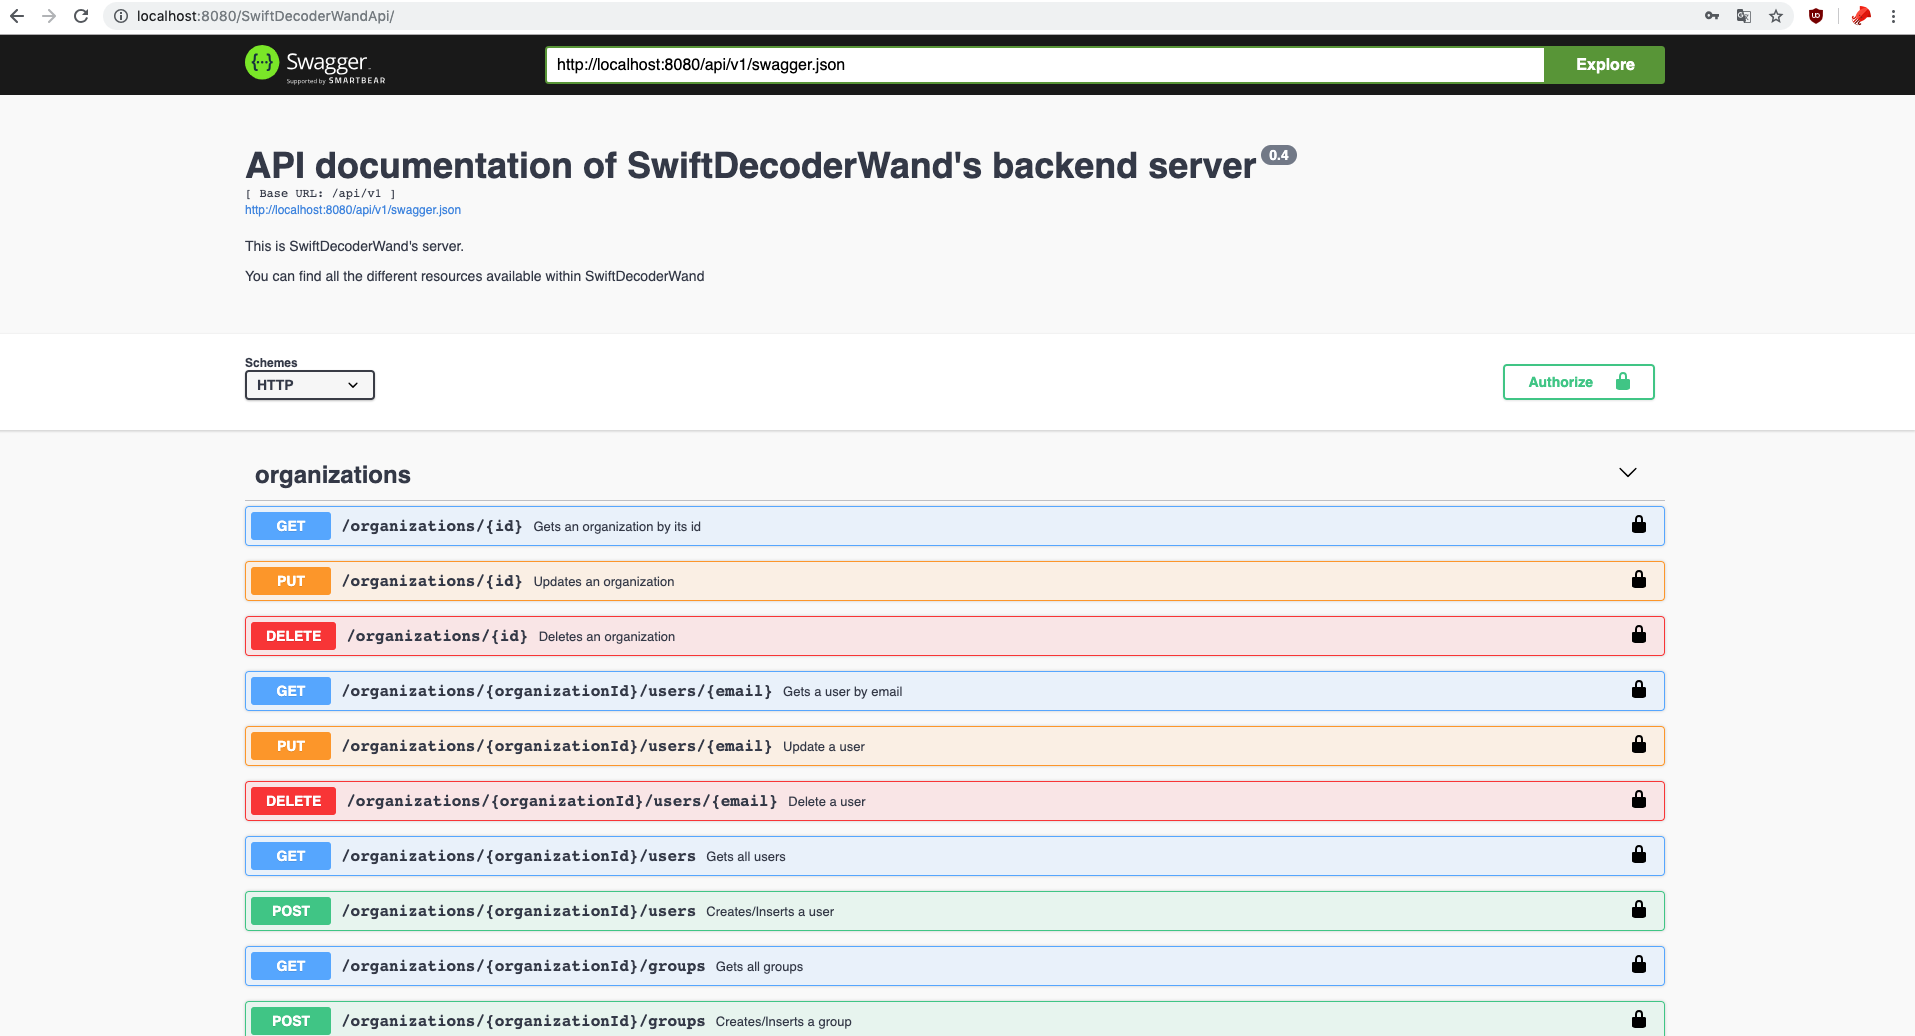
\includegraphics[scale = 0.2]{api.png}
				\caption{Documentation de l'API du backend}
			\end{figure}

			Le projet est en stade de recette et se termine début 2020, les parties frontend, mobiles et backend sont terminés et livrés, il ne subsiste seulement quelques améliorations selon le besoin du client et la livraison de la documentation dont j'ai eu la charge.

		\newpage

		\section{Formation Docker, Kubernetes}

		Au cours de cette année de formation, mon tuteur m'a confié la charge de réaliser une formation pour une entreprise.
		A travers le projet précedent, j'ai acquéris de nombreuses compétence sur la conteneurisation avec Docker.

		Ainsi j'ai pu donné une formation de 3 jours au sein de Docdoku autour de Docker. Il s'agit d'une présentation de la technologies, de toutes les briques de savoir nécessaire et de nombreux TP à réaliser.

		Egalement, j'ai pu réaliser le document de formation de Kubernetes, un outils Google de clusterisation des conteneurs docker.

			\begin{figure}[!htb]
				\center
				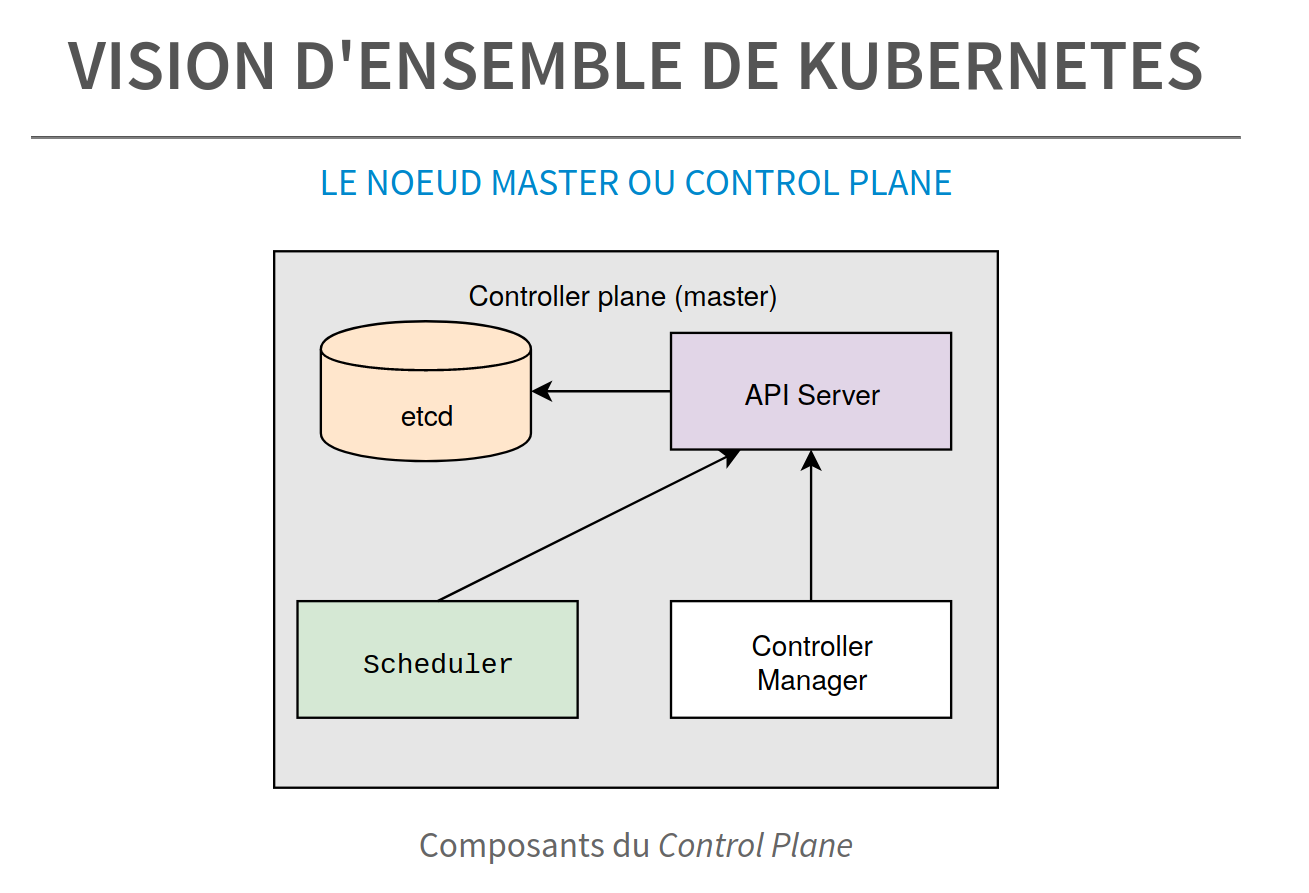
\includegraphics[scale = 0.2]{k8s.png}
				\caption{Formation kubernetes}
			\end{figure}

\end{document}